\documentclass[xcolor=svgnames]{beamer}
\mode<presentation>
{
      \setbeamertemplate{footline}[page number]
      \setbeamercovered{transparent}
      \setbeamertemplate{navigation symbols}{}
      \usecolortheme[named=DarkGreen]{structure}
}

\usepackage[english]{babel}
\usepackage{times}
\usepackage{url}
\usepackage{CJKutf8}
\usepackage{graphics}
\usepackage{amsmath}
\usepackage{listings}
\lstset{breakatwhitespace,
language=C++,
columns=fullflexible,
keepspaces,
breaklines,
tabsize=3,
showstringspaces=false,
extendedchars=true}


\begin{document}
\begin{CJK*}{UTF8}{gbsn}


\title{OS概念与Linux内核源代码分析之1}

\begin{frame}
\maketitle
\end{frame}

\defverbatim[colored]\lstdemo{
\begin{lstlisting}[tabsize=8,basicstyle=\ttfamily]
const char *processing() const{
            somestring = "-1";
}
\end{lstlisting}
}

%\begin{frame}{test}
%\lstdemo
%\end{frame}

\begin{frame}[fragile]
\frametitle{本课程Linux内核版本}
\begin{itemize}
\item linux kernel: 2.6.11.12 
\item 为什么使用这个版本的内核?
\item 下载地址: \url{http://www.kernel.org/pub/linux/kernel/v2.6}
\end{itemize}
\end{frame}

\begin{frame}[fragile]%{Linux内核关键数据结构:list}
\frametitle{Linux内核整体架构}
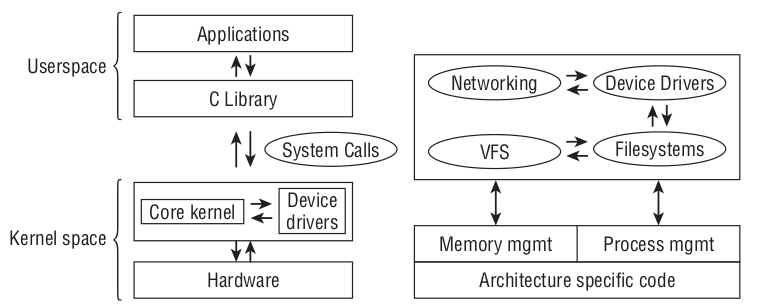
\includegraphics[width=1.0\textwidth]{kernel.png}
\end{frame}

\defverbatim[colored]\lstlisthead{
\begin{lstlisting}[tabsize=8,basicstyle=\ttfamily]
struct list_head {
        struct list_head *next, *prev;
};
\end{lstlisting}
}
\defverbatim[colored]\lstlistheadusage{
\begin{lstlisting}[tabsize=8,basicstyle=\ttfamily]
struct task_struct {
    ...
    struct list_head run_list;
    ...
};
\end{lstlisting}
}
\begin{frame}[fragile]%{Linux内核关键数据结构:list}
\frametitle{Linux内核关键数据结构:list}
\begin{block}{list\_head的定义: include/linux/list.h}
\lstlisthead
\end{block}
\begin{block}{list\_head的使用方法: include/linux/sched.h}
\lstlistheadusage
\end{block}
\end{frame}

\defverbatim[colored]\lstPCBstate{
\begin{lstlisting}[tabsize=8,basicstyle=\ttfamily]
struct task_struct {
        volatile long state;   
        ...
};
\end{lstlisting}
}
\defverbatim[colored]\lststates{
\begin{lstlisting}[tabsize=8,basicstyle=\ttfamily]
#define TASK_RUNNING        0
#define TASK_INTERRUPTIBLE  1
#define TASK_UNINTERRUPTIBLE    2
#define TASK_STOPPED        4
#define TASK_TRACED     8
#define TASK_DEAD       64
\end{lstlisting}
}

\defverbatim[colored]\lstinit{
\begin{lstlisting}[tabsize=8,basicstyle=\ttfamily]
#define LIST_HEAD_INIT(name) \
        { &(name), &(name) }

#define LIST_HEAD(name) \
    struct list_head name = LIST_HEAD_INIT(name)
\end{lstlisting}
}
\begin{frame}[fragile]
\frametitle{Linux内核关键数据结构:list}
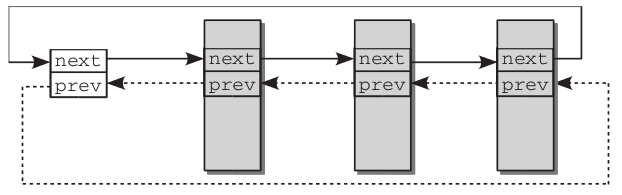
\includegraphics[width=1.0\textwidth]{list.png}
\begin{block}{list\_head结构的静态初始化: include/linux/list.h}
\lstinit
\end{block}
\end{frame}

\begin{frame}{针对list结构的操作}
\begin{itemize}
\item \alert{list\_add}(new, head) 把new插入head后面
\item \alert{list\_add\_tail}(new, head) 把new插入head前面
\item \alert{list\_del}(entry) 把entry从链表中删除
\item \alert{list\_empty}(head) 判断链表head是否为空
\item \alert{list\_splice}(list, head) 合并list和head
\item \alert{list\_entry}(ptr, type, member) 计算包含ptr的结构体的地址
\item \alert{list\_for\_each}(pos, head) 遍历以head为头的链表
\end{itemize}
\end{frame}

\defverbatim[colored]\lstadd{
\begin{lstlisting}[tabsize=8,basicstyle=\ttfamily]
typedef struct list_head list_head;

static inline void list_add(list_head *newn, 
                            list_head *head)
{
        __list_add(newn, head, head->next);
}

static inline void __list_add(list_head *newn,
                  list_head *prev,
                  list_head *next)
{
        next->prev = newn;
        newn->next = next;
        newn->prev = prev;
        prev->next = newn;
}
\end{lstlisting}
}
\begin{frame}[fragile]
\frametitle{针对list结构的操作: 代码分析举例}
\lstadd
\end{frame}

\defverbatim[colored]\lstforeach{
\begin{lstlisting}[tabsize=8,basicstyle=\ttfamily]
struct list_head *p;

list_for_each(p, &list) {
    if (!condition) continue;
    return list_entry(p, struct task_struct, 
                      run_list);
}

return NULL;
\end{lstlisting}
}
\begin{frame}[fragile]
\frametitle{针对list结构的操作: 代码分析举例}
\lstforeach
%\begin{block}{练习}
%从源文件include/linux/list.h中找出并理解上述针对list的各种操作函数的定义。
%\end{block}
\end{frame}

\begin{frame}[fragile]
\frametitle{针对list结构的操作: 代码分析举例}
\begin{block}{课外练习}
从源文件include/linux/list.h中找出上述list操作的函数代码,阅读并理解其实现。
\end{block}
\end{frame}

\defverbatim[colored]\lsthlist{
\begin{lstlisting}[tabsize=8,basicstyle=\ttfamily]
struct hlist_head {
        struct hlist_node *first;
};

struct hlist_node {
        struct hlist_node *next, **pprev;
};
\end{lstlisting}
}
\begin{frame}[fragile]
\frametitle{Linux内核关键数据结构:hlist\_head与hlist\_node}
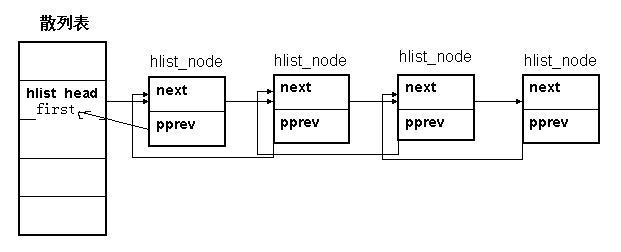
\includegraphics[width=0.9\textwidth]{hlist.jpeg}
\begin{block}{用于实现散列表:include/linux/list.h}
\lsthlist
\end{block}
\end{frame}

\begin{frame}%{Linux进程描述符: Process Descriptor}
\frametitle{Linux内核关键数据结构:hlist\_head与hlist\_node}
\begin{block}{思考及课外练习}
阅读include/linux/list.h中\alert{hlist\_add\_head}(), \alert{hlist\_del}(), \alert{hlist\_empty}(),
\alert{hlist\_add\_before}()等函数的实现,思考:

\begin{enumerate}
\item hlist\_node中的pprev字段指向什么内容?
\item[]
\item 为什么pprev采用二重指针?
\item[]
\item 为什么hlist\_head中只有一个成员first?
\end{enumerate}
\end{block}
\end{frame}

\defverbatim[colored]\lsttasks{
\begin{lstlisting}[tabsize=8,basicstyle=\ttfamily]
struct task_struct {
    ...
    struct list_head tasks;
    ...
};
\end{lstlisting}
}
\begin{frame}{Linux进程描述符: Process Descriptor}
\begin{block}{task\_struct结构: include/linux/sched.h}
\lsttasks
\end{block}
\begin{block}{系统中所有进程组成的链表}
%\lststates
以init\_task为表头,进程描述符的tasks字段将所有进程连接起来
\end{block}
\begin{block}{遍历系统中所有进程的宏: for\_each\_process}
阅读并理解include/linux/sched.h中for\_each\_process的实现。
\end{block}
\end{frame}

\defverbatim[colored]\lstrunning{
\begin{lstlisting}[tabsize=8,basicstyle=\ttfamily]
struct task_struct {
    ...
    int prio, static_prio;
    struct list_head run_list;
    prio_array_t *array;
    ...
};
\end{lstlisting}
}
\begin{frame}{Linux进程描述符: Process Descriptor}
\lstrunning
\begin{block}{各字段的含义}
\begin{itemize}
\item prio 为进程当前优先级 (0 -- 139)
\item run\_list 用于连接所有相同优先级的进程
\item array?
\end{itemize}
\end{block}
\end{frame}

\defverbatim[colored]\lstprio{
\begin{lstlisting}[tabsize=8,basicstyle=\ttfamily]
struct prio_array {
    unsigned int nr_active;
    unsigned long bitmap[BITMAP_SIZE];
    struct list_head queue[MAX_PRIO];
};
\end{lstlisting}
}
\begin{frame}{Linux进程描述符: Process Descriptor}
\begin{block}{kernel/sched.c}
\lstprio
\end{block}
\begin{block}{各成员字段的含义}
\begin{itemize}
\item nr\_active: 当前列表中进程总数
\item bitmap 用于记录哪个队列为非空
\item queue用于存储140个队列的表头
\end{itemize}
\end{block}
\end{frame}

\begin{frame}{课外练习}
上页中,\alert{BITMAP\_SIZE}和\alert{MAX\_PRIO}两个宏分别在文件kernel/sched.c和include/linux/sched.h中定义,请确定这两个宏
的具体数值。
\end{frame}

\begin{frame}{Linux进程描述符: Process Descriptor}
\begin{block}{task\_struct结构: include/linux/sched.h}
\lstPCBstate
\end{block}
\begin{block}{进程可能的状态: include/linux/sched.h}
\lststates
\end{block}
\end{frame}

\begin{frame}{Linux进程描述符: Process Descriptor}
\begin{block}{改变进程状态的函数/宏}
\begin{itemize}
\item set\_task\_state 改变指定进程的状态
\item set\_current\_state 改变当前执行的进程的状态
\end{itemize}
\end{block}
\begin{block}{课外练习}
阅读以上两个函数的源代码(位于文件include/linux/sched.h),并思考为什么要这样写。
\end{block}
\end{frame}

%\begin{frame}[fragile]%{Linux内核关键数据结构:list}
%\frametitle{进程与线程的区别与联系}
%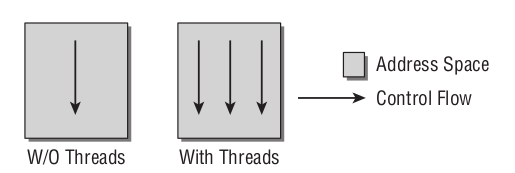
\includegraphics[width=1.0\textwidth]{proc_thread.png}
%\begin{itemize}
%\item 进程是资源分配单位(地址空间、I/O等资源)
%\item 线程是执行单位
%\end{itemize}
%\end{frame}

%\begin{frame}[fragile]%{Linux内核关键数据结构:list}
%\frametitle{Linux中的内核地址空间与用户地址空间}
%\begin{columns}%[b]
%\column{.4\textwidth}
%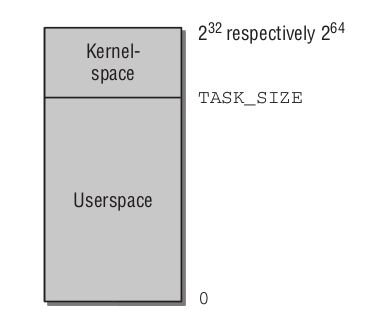
\includegraphics[width=1.0\textwidth]{as.png}
%\column{.6\textwidth}
%\begin{itemize}
%\item 用户地址空间从0到TASK\_SIZE-1
%\item 内核地址空间从TASK\_SIZE到$2^{32}$-1
%\end{itemize}
%\end{columns}
%\end{frame}
%
%\begin{frame}[fragile]%{Linux内核关键数据结构:list}
%\frametitle{Linux中的内核地址空间与用户地址空间}
%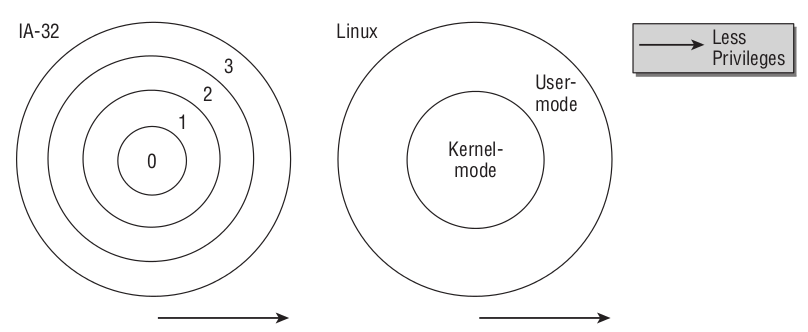
\includegraphics[width=1.0\textwidth]{ring.png}
%\begin{itemize}
%\item 用户态下只能访问用户地址空间
%\item 核心态下可以访问所有地址空间
%\item 二者其他区别?
%\end{itemize}
%\end{frame}

%\begin{frame}[fragile]%{Linux内核关键数据结构:list}
%\frametitle{分页技术与地址空间共享}
%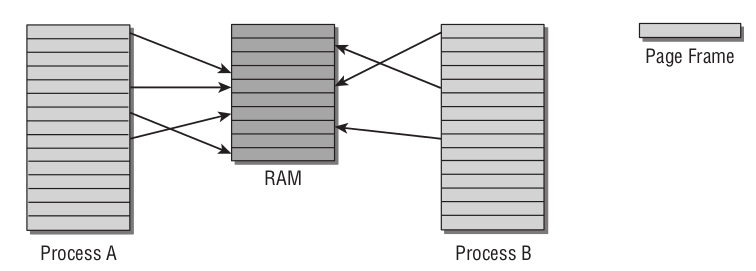
\includegraphics[width=1.0\textwidth]{paging.png}
%
%注意观察A、B进程的第0页面对应的物理页框;地址空间的共享(代码、数据)
%\end{frame}

%\begin{frame}[fragile]%{Linux内核关键数据结构:list}
%\frametitle{Linux下的多级分页技术}
%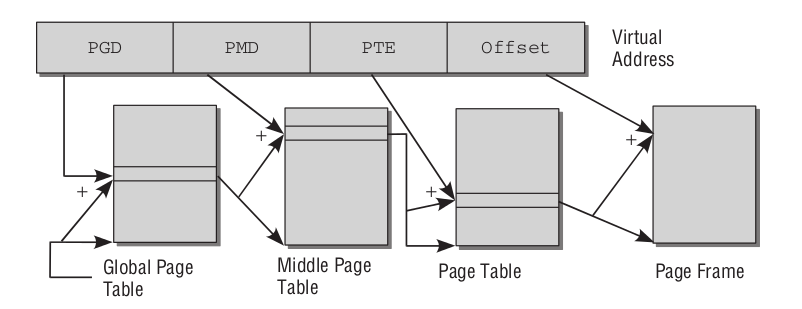
\includegraphics[width=1.0\textwidth]{pagetables.png}
%
%CPU内部进行地址映射的两个硬件单元:MMU/TLB
%\end{frame}

%\begin{frame}[fragile]%{Linux内核关键数据结构:list}
%\frametitle{物理内存的分配算法:伙伴系统}
%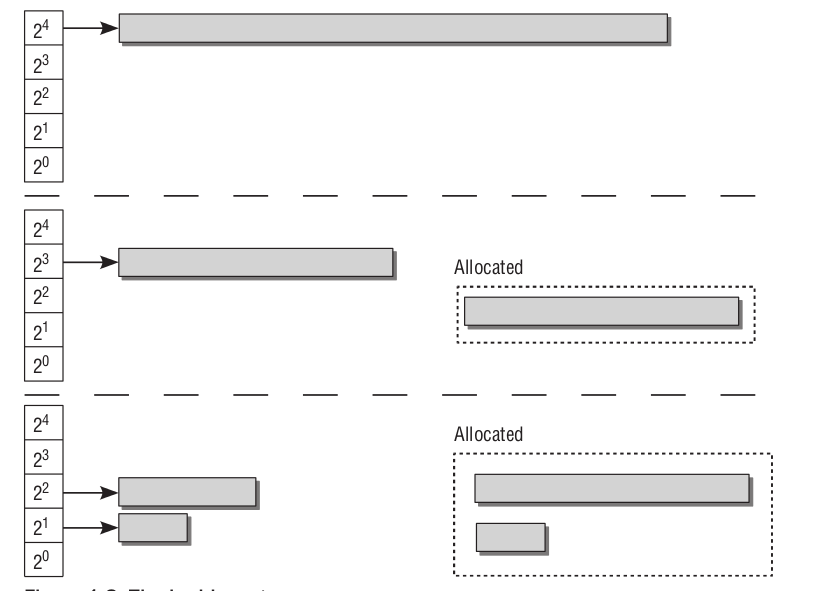
\includegraphics[width=0.8\textwidth]{buddy.png}

%注意观察A、B进程的第0页面对应的物理页框;地址空间的共享(代码、数据)
%\end{frame}



\begin{frame}[fragile]
\frametitle{Linux进程表示:task\_struct结构}
\begin{block}{include/linux/sched.h}
\begin{verbatim}
struct task_struct {
    volatile long state;    /* -1 unrunnable */
    void *stack;
    atomic_t usage;
    unsigned int flags; /* per process flags */
    unsigned int ptrace;

    int lock_depth;     /* BKL lock depth */

#ifdef CONFIG_SMP
#ifdef __ARCH_WANT_UNLOCKED_CTXSW
    int oncpu;
#endif
#endif
    ...
};


\end{verbatim}
\end{block}
\end{frame}

%\begin{frame}[fragile]
%\frametitle{Linux进程表示:task\_struct结构}
%\begin{block}{task\_struct结构的state字段}
%\begin{verbatim}
%\end{verbatim}
%\end{block}
%\end{frame}

\begin{frame}[fragile]
\frametitle{Linux进程表示:task\_struct结构}
\begin{block}{task\_struct结构的rlim字段: include/linux/resource.h}
\begin{verbatim}
struct rlimit {
    unsigned long   rlim_cur;
    unsigned long   rlim_max;
};

struct task_struct {
    ...
    struct rlimit rlim[RLIM_NLIMITS];
    ...
};
\end{verbatim}
\end{block}
\begin{block}{相关系统调用:}
\begin{verbatim}
int getrlimit(int res, struct rlimit *rlim);
int setrlimit(int res, const struct rlimit *rlim);
\end{verbatim}
\end{block}
\end{frame}

\begin{frame}[fragile]
\frametitle{Linux进程表示:task\_struct结构}
\begin{block}{task\_struct结构的rlim字段: include/asm-generic/resource.h}
\begin{verbatim}
#define RLIMIT_CPU      0   
#define RLIMIT_FSIZE        1  
#define RLIMIT_DATA     2   
#define RLIMIT_STACK        3 
#define RLIMIT_CORE     4   
#define RLIMIT_NOFILE      7  
...
#define RLIM_NLIMITS        15
\end{verbatim}
\end{block}
\begin{block}{相关命令}
cat /proc/self/limits
\end{block}
\end{frame}

\begin{frame}{名字空间(namespaces)的概念}

传统UNIX只有唯一的名字空间:

\begin{description}
\item[PID] 进程编号
\item[UID] 用户编号
\item[GID] 群组编号
\end{description}

\begin{block}{唯一名字空间的缺点举例}
计算服务提供商:希望为用户提供Linux操作系统的使用服务,每个用户都可以拥有root权限。
\end{block}

\begin{block}{解决方法}
\begin{itemize}
\item 每个用户一台机器?
\item 虚拟机(VMWare)?
\end{itemize}
\end{block}

\end{frame}

\begin{frame}{名字空间(namespaces)的概念}
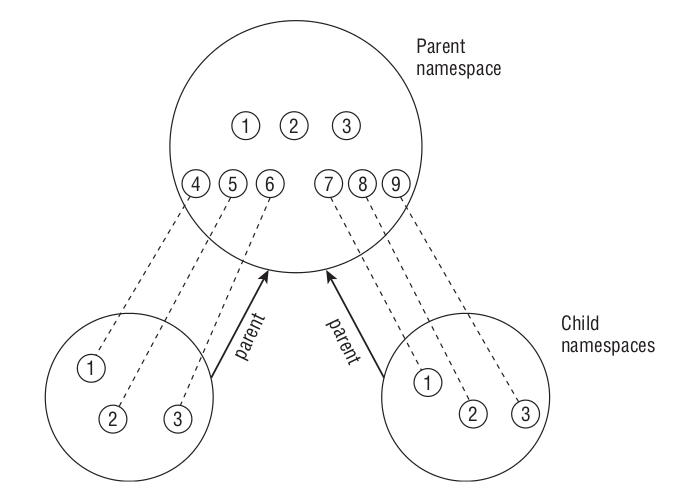
\includegraphics[width=0.9\textwidth]{ns.png}
\begin{block}{名字空间的相互关系}
上图中,子名字空间中的1,2,3编号与父名字空间中的1,2,3完全不相关
\end{block}
\end{frame}

\begin{frame}[fragile]
\frametitle{Linux内核中名字空间的实现}
\begin{block}{struct nsproxy: 按照功能划分若干名字空间 -- include/linux/nsproxy.h}
\begin{verbatim}
struct nsproxy {
    atomic_t count;
    struct uts_namespace *uts_ns;
    struct ipc_namespace *ipc_ns;
    struct mnt_namespace *mnt_ns;
    struct pid_namespace *pid_ns;
    struct user_namespace *user_ns;
    struct net       *net_ns;
};
\end{verbatim}
\end{block}
\end{frame}

\begin{frame}[fragile]
\frametitle{Linux内核中名字空间的实现}
\begin{block}{struct nsproxy: 按照功能划分若干名字空间 -- include/linux/sched.h}
\begin{verbatim}
struct task_struct {
    ...
    struct nsproxy *nsproxy;
    ...
}
\end{verbatim}
\end{block}
\end{frame}

\begin{frame}{Linux内核中名字空间的实现}
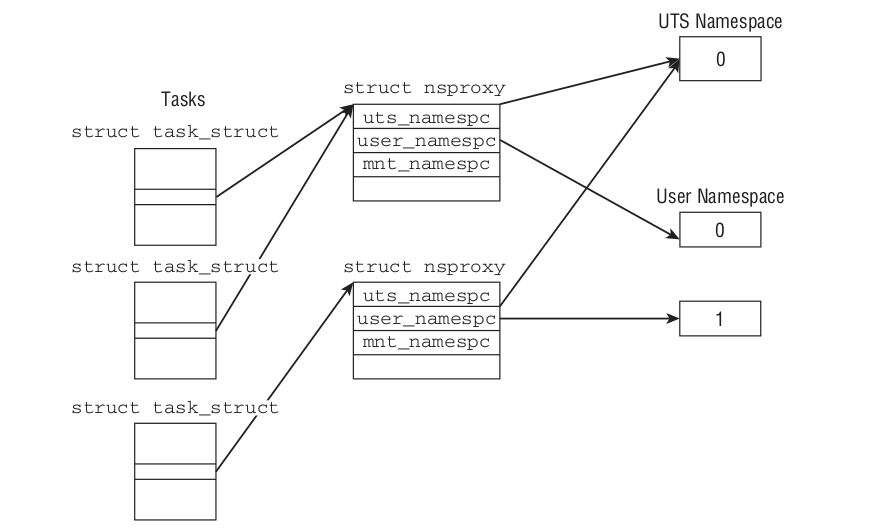
\includegraphics[width=0.9\textwidth]{ns_impl.png}
\end{frame}

\begin{frame}[fragile]
\frametitle{Linux内核中名字空间的实现}
\begin{block}{fork新进程时可以指明是否为此进程建立新的名字空间:}
\begin{verbatim}
#define CLONE_NEWUTS    0x04000000  
#define CLONE_NEWIPC    0x08000000 
#define CLONE_NEWUSER   0x10000000
#define CLONE_NEWPID    0x20000000
#define CLONE_NEWNET    0x40000000 
\end{verbatim}
\end{block}
\end{frame}

\begin{frame}[fragile]
\frametitle{初始全局名字空间的定义}
\begin{block}{kernel/nsproxy.c}
\begin{verbatim}
struct nsproxy init_nsproxy = \
       INIT_NSPROXY(init_nsproxy);
\end{verbatim}
\end{block}
\begin{block}{include/linux/init\_task.h}
\begin{verbatim}
#define INIT_NSPROXY(nsproxy) {                     \
    .pid_ns     = &init_pid_ns,                 \
    .count      = ATOMIC_INIT(1),               \
    .uts_ns     = &init_uts_ns,                 \
    .mnt_ns     = NULL,                     \
    INIT_NET_NS(net_ns)                                             \
    INIT_IPC_NS(ipc_ns)                     \
    .user_ns    = &init_user_ns,                \
}

\end{verbatim}
\end{block}
\end{frame}

\begin{frame}[fragile]
\frametitle{UTS Namespace}
\begin{block}{include/linux/utsname.h}
\begin{verbatim}
struct uts_namespace {
    struct kref kref;
    struct new_utsname name;
};

struct new_utsname {
    char sysname[65];
    char nodename[65];
    char release[65];
    char version[65];
    char machine[65];
    char domainname[65];
};
\end{verbatim}
\end{block}
\end{frame}
\begin{frame}[fragile]
\frametitle{UTS Namespace的初始值}
\begin{block}{init/version.c}
\begin{verbatim}
struct uts_namespace init_uts_ns = {
    .kref = {
        .refcount   = ATOMIC_INIT(2),
    },
    .name = {
        .sysname    = UTS_SYSNAME,
        .nodename   = UTS_NODENAME,
        .release    = UTS_RELEASE,
        .version    = UTS_VERSION,
        .machine    = UTS_MACHINE,
        .domainname = UTS_DOMAINNAME,
    },
};
\end{verbatim}
\end{block}
\end{frame}

\begin{frame}[fragile]
\frametitle{User Namespace}
\begin{block}{include/linux/user\_namespace.h}
\begin{verbatim}
struct user_namespace {
    struct kref kref;
    struct hlist_head uidhash_table[UIDHASH_SZ];
    struct user_struct *root_user;
};
\end{verbatim}
\end{block}
\end{frame}

\begin{frame}[fragile]
\frametitle{进程间的相互关系}
\begin{block}{include/linux/sched.h}
\begin{verbatim}
struct task_struct {
    ...
    struct list_head children; /* children list */
    struct list_head sibling; /* parent’s children list */
    ...
}
\end{verbatim}
\end{block}
\end{frame}

\begin{frame}{进程间的相互关系}
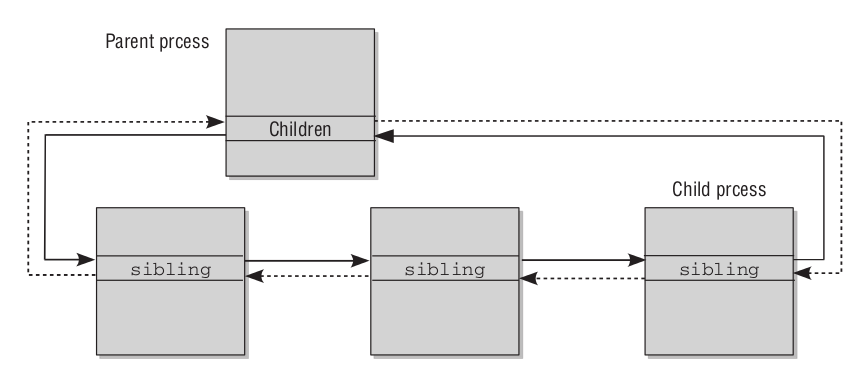
\includegraphics[width=1.0\textwidth]{parent.png}
\begin{block}{children与sibling}
\begin{itemize}
\item children是指向本进程所有子进程的链表表头
\item sibling用于连接兄弟进程
\item pstree命令显示进程结构树(用途?)
\end{itemize}
\end{block}
\end{frame}

\begin{frame}{创建进程的系统调用}
\begin{enumerate}
\item fork用于创建新进程
\item[]
\item vfork创建新进程,并且只有当子进程运行完毕,父进程才能运行;二者共享存储空间(deprecated)
\item[]
\item clone用于创建进程或者线程

\end{enumerate}
\end{frame}

\begin{frame}{创建进程的系统调用: 写拷贝技术(copy-on-write)}
历史上,unix中调用fork创建新进程时,OS需要将父进程的存储空间完全拷贝一份给子进程,这有以下缺点:
\begin{itemize}
\item 拷贝内存的过程非常耗时
\item 需要占用大量内存空间
\item 子进程一旦执行exec,则上述拷贝完全浪费
\end{itemize}

写拷贝(copy-on-write): 创建新进程时,仅拷贝父进程的页表,并将所有页表项对应的页面设置成只读,只有当
父亲或子进程需要写入某页面时,才拷贝相应页面的内容。
\end{frame}

\begin{frame}[fragile]
\frametitle{创建进程: do\_fork函数}
\begin{block}{kernel/fork.c}
\begin{verbatim}
long do_fork(unsigned long clone_flags,
             unsigned long stack_start,
             struct pt_regs *regs,
             unsigned long stack_size,
             int __user *parent_tidptr,
             int __user *child_tidptr)
\end{verbatim}
\end{block}
\begin{itemize}
\item clone\_flags用于描述进程的哪些属性将被复制(进程/线程!)
\item start\_stack为用户态下进程的栈起始位置, stack\_size为栈的总长度
\item regs, parent\_tidptr等参数后面讲
\end{itemize}
\end{frame}

\begin{frame}[fragile]
\frametitle{创建进程: do\_fork函数}
\begin{block}{arch/x86/kernel/process\_32.c}
\begin{verbatim}
asmlinkage int sys_fork(struct pt_regs regs)
{
    return do_fork(SIGCHLD, regs.esp, &regs, 
                   0, NULL, NULL);
}
\end{verbatim}
\end{block}
\end{frame}

\begin{frame}[fragile]
\frametitle{创建进程: do\_fork函数}
\begin{block}{arch/x86/kernel/process\_32.c}
\begin{verbatim}
asmlinkage int sys_clone(struct pt_regs regs)
{
    unsigned long clone_flags;
    unsigned long newsp;
    int __user *parent_tidptr, *child_tidptr;
    clone_flags = regs.ebx;
    newsp = regs.ecx;
    parent_tidptr = (int __user *)regs.edx;
    child_tidptr = (int __user *)regs.edi;
    if (!newsp)
        newsp = regs.esp;
    return do_fork(clone_flags, newsp, &regs, 
                   0, parent_tidptr, child_tidptr);
}

\end{verbatim}
\end{block}
\end{frame}

%\begin{frame}[fragile]
%\frametitle{创建进程: do\_fork函数的实现}
%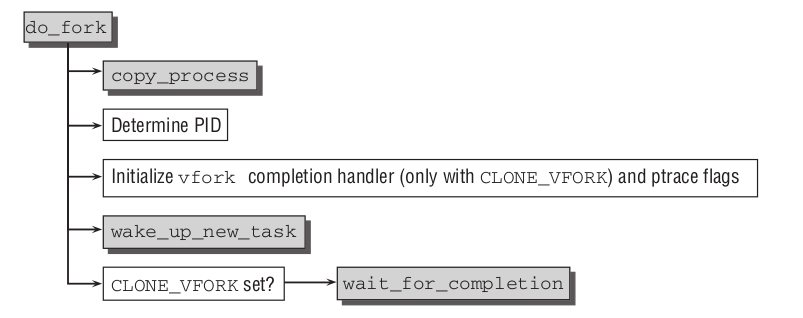
\includegraphics[width=1.0\textwidth]{dofork.png}
%\end{frame}

%\begin{frame}{操作系统中三个最重要的概念}
%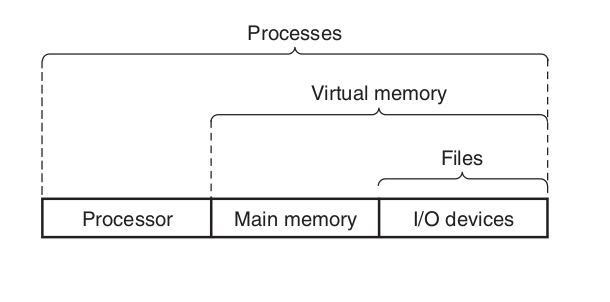
\includegraphics[width=1.0\textwidth]{osabstractions.png}
%\end{frame}


%\begin{frame}{对临界资源的互斥访问}
%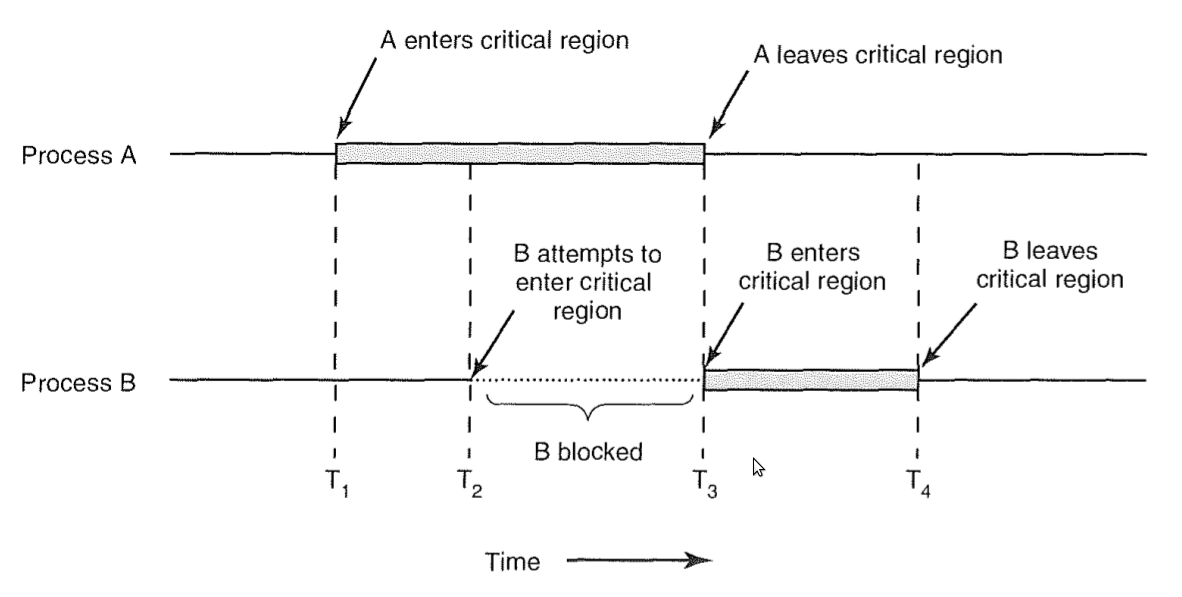
\includegraphics[width=1.0\textwidth]{mutual.png}
%\end{frame}

%\begin{frame}{用信号量解决生产者--消费者问题}
%\begin{columns}[b]
%\column{.5\textwidth}
%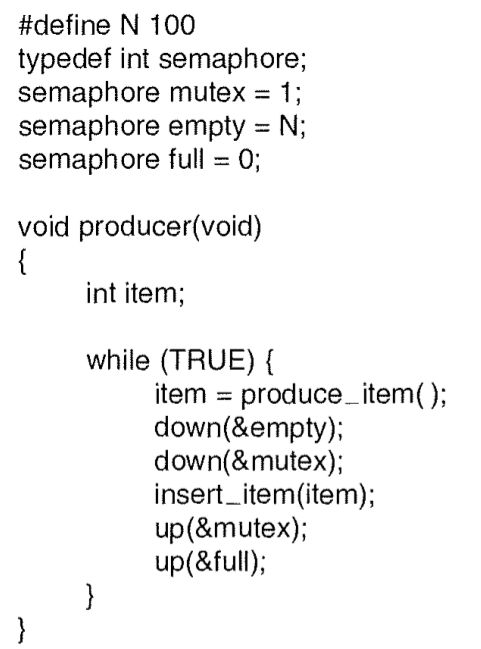
\includegraphics[width=1.0\textwidth]{prodsem.png}
%\column{.5\textwidth}
%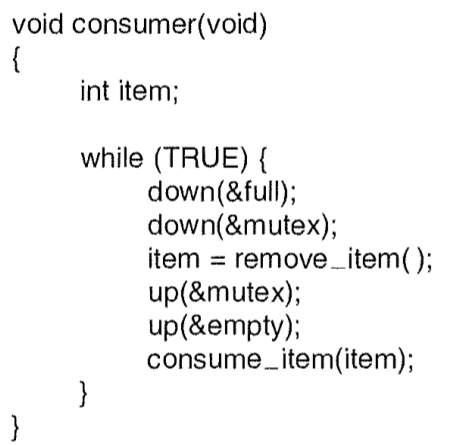
\includegraphics[width=1.0\textwidth]{conssem.png}
%\end{columns}%[t]

%该方案中,信号量empty和full具有计数和同步功能,而mutex仅有互斥功能。
%\end{frame}

%\begin{frame}{专门用来实现互斥的特殊信号量 -- 互斥锁}
%互斥锁只有两种状态:locked (1) / unlocked (0)
%
%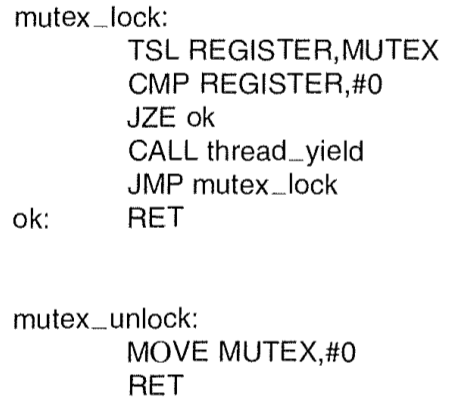
\includegraphics[width=0.5\textwidth]{mutex.png}
%\end{frame}

%\begin{frame}{互斥锁与忙等待的区别}
%\begin{columns}[b]
%\column{.5\textwidth}
%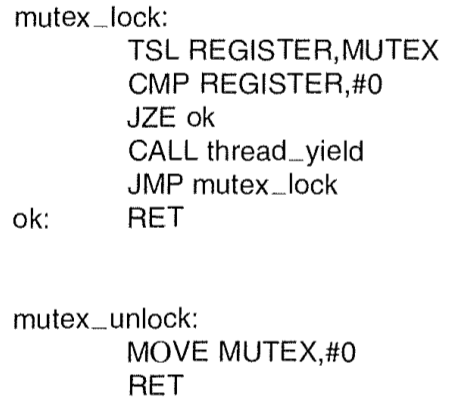
\includegraphics[width=1.0\textwidth]{mutex.png}
%\column{.5\textwidth}
%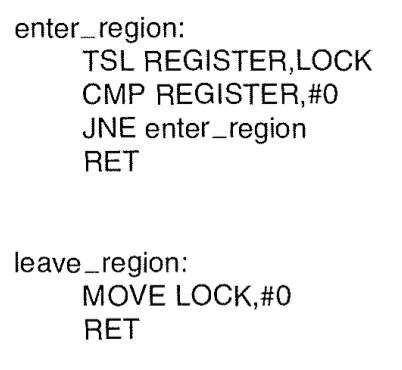
\includegraphics[width=1.0\textwidth]{tsl.png}
%\end{columns}%[t]
%后者:不断利用CPU指令测试临界资源,直至时间片用光被从CPU上撤下来
%\end{frame}
%
%\begin{frame}{信号量的危险情形 --- 管程机制的引入}
%\begin{columns}[b]
%\column{.5\textwidth}
%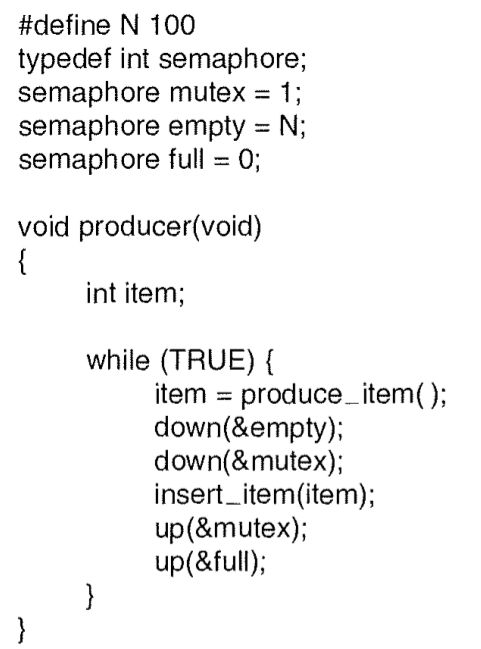
\includegraphics[width=1.0\textwidth]{prodsem.png}
%\column{.5\textwidth}
%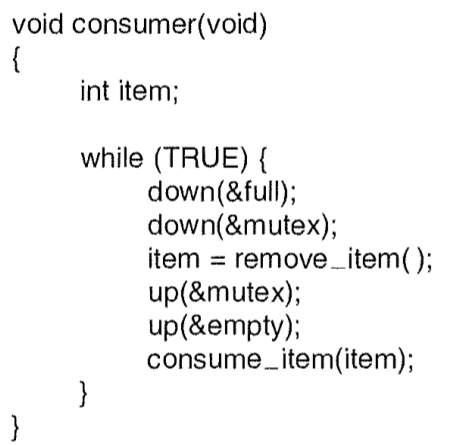
\includegraphics[width=1.0\textwidth]{conssem.png}
%\end{columns}%[t]
%\alert{危险:}如果程序员不小心把producer中的down(empty)和down(mutex)顺序颠倒,
%则当缓冲区满时,会发生什么?
%\end{frame}

%\begin{frame}{信号量的危险情形 --- 管程机制的引入}
%\begin{itemize}
%\item 发生死锁。
%\item[]
%\item 因此,最好由编译器自动处理这种容易出错的程序段。---引入管程。
%\item[]
%\item 对比:C++中构造函数与析构函数
%\end{itemize}
%\end{frame}

%\begin{frame}{管程:解决生产者--消费者问题}
%\begin{columns}[b]
%\column{.5\textwidth}
%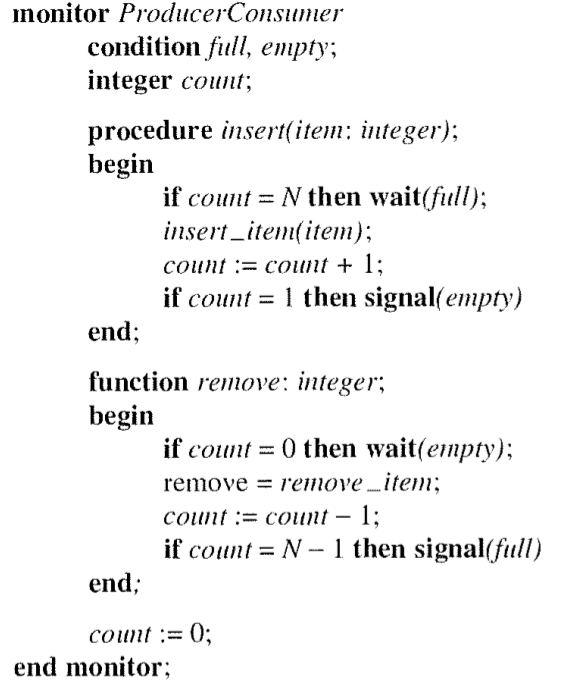
\includegraphics[width=1.0\textwidth]{mon1.png}
%\column{.5\textwidth}
%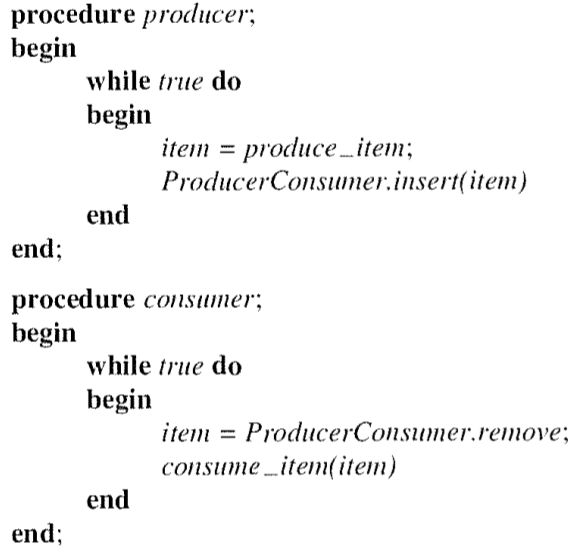
\includegraphics[width=1.0\textwidth]{mon2.png}
%\end{columns}%[t]
%
%\alert{注意概念:} 条件变量empty, full以及wait, signal
%
%此外,insert与remove之间的互斥由编译器完成
%\end{frame}

%\begin{frame}{管程:解决生产者--消费者问题}
%\begin{itemize}
%\item 管程内程序段之间的互斥(自动)
%\item 进程同步问题?:条件变量及wait, signal实现
%\begin{itemize}
%\item wait: 将当前进程阻塞,并允许其他进程进入管程
%\item signal: 将被相应条件变量阻塞的进程唤醒
%%\end{itemize}
%\item 上述方法中,signal必须是最后一条指令,为什么? 
%\end{itemize}
%\end{frame}

%\begin{frame}{消息传递机制:解决不同机器上进程间同步问题}
%\begin{columns}[b]
%\column{.5\textwidth}
%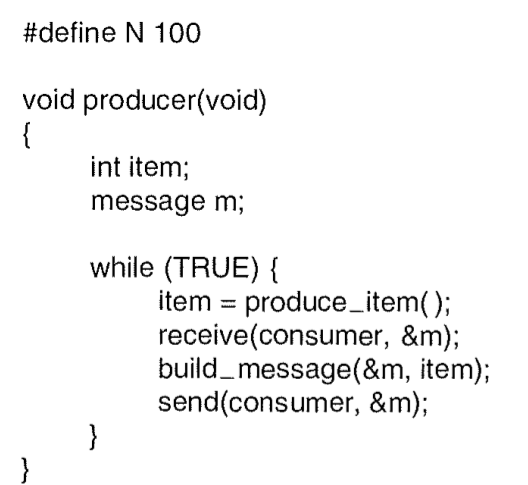
\includegraphics[width=1.0\textwidth]{msgprod.png}
%\column{.5\textwidth}
%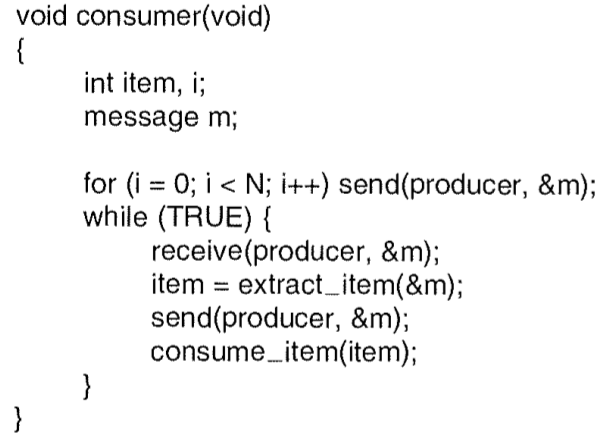
\includegraphics[width=1.0\textwidth]{msgcons.png}
%\end{columns}%[t]
%\end{frame}


\end{CJK*}
\end{document}
